
\section {Python Modules}

\vspace{\baselineskip}
\noindent Modul memungkinkan Anda mengatur kode Python secara logis. Mengelompokkan kode terkait ke dalam modul membuat kode lebih mudah dipahami dan digunakan. Modul adalah objek Python dengan atribut yang diberi nama sewenang-wenang sehingga Anda bisa mengikat dan memberi referensi.\par
\vspace{\baselineskip}
\noindent Cukup, modul adalah file yang terdiri dari kode Python. Modul dapat mendefinisikan fungsi, kelas dan variabel. Modul juga bisa menyertakan kode runnable.\par


\vspace{\baselineskip}
\noindent Example\par
\vspace{\baselineskip}
\noindent Kode Python untuk sebuah modul bernama aname biasanya berada pada sebuah file bernama aname.py. Berikut adalah contoh modul sederhana, support.py\par

\vspace{\baselineskip}
\begin{verbatim}


def print_func( par ):
print "Hello : ", par
return

\end{verbatim}

\begin{itemize}
	\item The import Statement
\end{itemize}
\noindent Anda dapat menggunakan file sumber Python apapun sebagai modul dengan mengeksekusi pernyataan impor di file sumber Python lainnya. Impor memiliki sintaks berikut:\par


\vspace{\baselineskip}
\noindent import module1[, module2[,... moduleN]\par


\vspace{\baselineskip}
\noindent Ketika penafsir menemukan sebuah pernyataan impor, ia mengimpor modul jika modul tersebut ada di jalur pencarian. Jalur pencarian adalah daftar direktori yang ditafsirkan juru bahasa sebelum mengimpor modul. Misalnya, untuk mengimpor modul support.py, Anda perlu meletakkan perintah berikut di bagian atas skrip -\par

\vspace{\baselineskip}
\begin{verbatim}

# !/usr/bin/python
# Import module support
import support

\end{verbatim}

\vspace{\baselineskip}
\noindent $\#$  Now you can call defined function that module as follows\par

\noindent support.print$ \_ $ func("Zara")\par

\vspace{\baselineskip}
\noindent Bila kode diatas dieksekusi, maka menghasilkan hasil sebagai berikut -\par
\vspace{\baselineskip}
\noindent Hello : Zara\par

\vspace{\baselineskip}
\noindent Modul hanya dimuat satu kali, berapa pun jumlahnya diimpor. Hal ini mencegah eksekusi modul terjadi berulang-ulang jika terjadi beberapa impor.\par

\vspace{\baselineskip}
\noindent The from...import Statement\par

\vspace{\baselineskip}
\noindent Python dari pernyataan memungkinkan Anda mengimpor atribut tertentu dari modul ke dalam namespace saat ini. Dari ... impor memiliki sintaks berikut -\par


\vspace{\baselineskip}
\noindent from modname import name1[, name2[, ... nameN]]\par


\vspace{\baselineskip}
\noindent Misalnya, untuk mengimpor fungsi fibonacci dari modul fib, gunakan pernyataan berikut -\par

\vspace{\baselineskip}
\vspace{\baselineskip}
\noindent from fib import fibonacci\par

\vspace{\baselineskip}
\noindent Pernyataan ini tidak mengimpor seluruh modul fib ke dalam namespace saat ini; Itu hanya memperkenalkan item fibonacci dari modul fib ke dalam tabel simbol global modul pengimpor.\par


\vspace{\baselineskip}
\begin{itemize}
	\item The from...import * Statement:
\end{itemize}

\noindent Hal ini juga memungkinkan untuk mengimpor semua nama dari modul ke dalam namespace saat ini dengan menggunakan pernyataan impor berikut -\par


\vspace{\baselineskip}
\noindent from modname import *\par


\vspace{\baselineskip}
\noindent Ini menyediakan cara mudah untuk mengimpor semua item dari modul ke dalam namespace saat ini; Namun, pernyataan ini harus digunakan dengan hemat.\par


\vspace{\baselineskip}
\begin{itemize}
	\item Locating Modules
\end{itemize}

\noindent Saat mengimpor modul, juru bahasa Python mencari modul dalam urutan berikut -\par

\vspace{\baselineskip}
$\bullet$  Direktori saat ini.\par

\vspace{\baselineskip}
$\bullet$  Jika modul tidak ditemukan, Python kemudian mencari setiap direktori di variabel shell PYTHONPATH.\par

\vspace{\baselineskip}
$\bullet$  Jika semuanya gagal, Python memeriksa jalur default. Di UNIX, jalur default ini biasanya / usr / local / lib / python /.\par


\vspace{\baselineskip}
\noindent Jalur pencarian modul disimpan dalam sistem modul sys sebagai sys.pathvariable. Variabel sys.path berisi direktori saat ini, PYTHONPATH, dan default pengaturan instalasi.\par

\vspace{\baselineskip}
\vspace{\baselineskip}
\noindent The PYTHONPATH Variable:\par

\vspace{\baselineskip}
\noindent The PYTHONPATH adalah variabel lingkungan, yang terdiri dari daftar direktori. Sintaksis PYTHONPATH sama dengan variabel shell PATH.\par

\vspace{\baselineskip}
\noindent Berikut adalah PYTHONPATH khas dari sistem Windows:\par
\noindent \hspace*{0.5in}set PYTHONPATH=c:$\textbackslash$ python20$\textbackslash$ lib;\par
\vspace{\baselineskip}
\noindent Dan berikut ini adalah PYTHONPATH khas dari sistem UNIX:\par
\noindent \hspace*{0.5in}set PYTHONPATH=/usr/local/lib/python\par


\vspace{\baselineskip}
\begin{itemize}
	\item Namespaces and Scoping
\end{itemize}

\noindent Variabel adalah nama (identifiers) yang memetakan ke objek. Namespace adalah kamus dari nama variabel (kunci) dan objek yang sesuai (nilai).\par

\vspace{\baselineskip}
\noindent Pernyataan Python dapat mengakses variabel dalam namespace lokal dan dalam namespace global. Jika variabel lokal dan global memiliki nama yang sama, variabel lokal membayangi variabel global. Setiap fungsi memiliki namespace lokal sendiri. Metode kelas mengikuti aturan pelingkupan yang sama dengan fungsi biasa.\par

\vspace{\baselineskip}
\noindent Python membuat tebakan terdidik tentang apakah variabel bersifat lokal atau global. Ini mengasumsikan bahwa setiap variabel yang diberi nilai dalam suatu fungsi adalah lokal.\par
\vspace{\baselineskip}
\noindent Oleh karena itu, untuk menetapkan nilai pada variabel global dalam suatu fungsi, Anda harus terlebih dahulu menggunakan pernyataan global.\par

\vspace{\baselineskip}
\noindent Pernyataan global VarName memberitahu Python bahwa VarName adalah variabel global. Python berhenti mencari namespace lokal untuk variabel tersebut.\par

\vspace{\baselineskip}
\noindent Sebagai contoh, kita mendefinisikan sebuah variabel Money in the global namespace. Dalam fungsi Money, kita menetapkan Money a value, oleh karena itu Python mengasumsikan variabel lokal Moneyas. Namun, kami mengakses nilai variabel lokal Moneybefore yang mengaturnya, jadi UnboundLocalError adalah hasilnya. Uncommenting pernyataan global memperbaiki masalahnya.\par
\vspace{\baselineskip}
\hspace*{0.5in}
\vspace{\baselineskip}
\noindent $\#$ !/usr/bin/python\par


\noindent \hspace*{0.5in}Money = 2000\par


\noindent \hspace*{0.5in}def AddMoney():\par


\noindent \hspace*{0.5in}~~ $\#$  Uncomment the following line to fix the code:\par


\noindent \hspace*{0.5in}~~ $\#$  global Money\par


\noindent \hspace*{0.5in}~~ Money = Money + 1\par


\vspace{\baselineskip}
\noindent \hspace*{0.5in}print Money\par


\noindent \hspace*{0.5in}AddMoney()\par


\noindent \hspace*{0.5in}print Money\par


\vspace{\baselineskip}
\begin{itemize}
	\item The dir( ) Function
\end{itemize}

\noindent Fungsi dir () built-in mengembalikan daftar string yang diurutkan yang berisi nama yang ditentukan oleh sebuah modul.\par


\noindent Daftar berisi nama semua modul, variabel dan fungsi yang didefinisikan dalam modul. Berikut adalah contoh sederhana -\par
\vspace{\baselineskip}

\begin{verbatim}

# !/usr/bin/python
# Import built-in module math
import math\par
content = dir(math)
print content

\end{verbatim}

\vspace{\baselineskip}
\noindent Bila kode diatas dieksekusi, maka menghasilkan hasil sebagai berikut -\par

\vspace{\baselineskip}
\noindent \hspace*{0.5in}['$ \_ $ $ \_ $ doc$ \_ $ $ \_ $ ', '$ \_ $ $ \_ $ file$ \_ $ $ \_ $ ', '$ \_ $ $ \_ $ name$ \_ $ $ \_ $ ', 'acos', 'asin', 'atan', \par


\noindent \hspace*{0.5in}'atan2', 'ceil', 'cos', 'cosh', 'degrees', 'e', 'exp', \par


\noindent \hspace*{0.5in}'fabs', 'floor', 'fmod', 'frexp', 'hypot', 'ldexp', 'log',\par


\noindent \hspace*{0.5in}'log10', 'modf', 'pi', 'pow', 'radians', 'sin', 'sinh', \par


\noindent \hspace*{0.5in}'sqrt', 'tan', 'tanh']\par

\vspace{\baselineskip}
\noindent Di sini, variabel string khusus $ \_ $ $ \_ $ name$ \_ $ $ \_ $  adalah nama modul, dan $ \_ $ $ \_ $ file$ \_ $ $ \_ $  adalah nama file tempat modul dimuat.\par


\vspace{\baselineskip}
\begin{itemize}
	\item The globals() and locals() Functions 
\end{itemize}

\noindent Fungsi global () dan penduduk lokal () dapat digunakan untuk mengembalikan nama di ruang nama global dan lokal tergantung pada lokasi dari tempat mereka dipanggil.\par

\vspace{\baselineskip}
\noindent Jika penduduk setempat () dipanggil dari dalam sebuah fungsi, maka semua nama yang dapat diakses secara lokal berasal dari fungsi itu.\par
\vspace{\baselineskip}
\noindent Jika globals () dipanggil dari dalam sebuah fungsi, maka akan mengembalikan semua nama yang dapat diakses secara global dari fungsi itu.\par
\vspace{\baselineskip}
\noindent Jenis kembalian dari kedua fungsi ini adalah kamus. Oleh karena itu, nama dapat diekstrak dengan menggunakan tombol () fungsi.\par


\vspace{\baselineskip}
\begin{itemize}
	\item The reload() Function
\end{itemize}

\noindent Saat modul diimpor ke dalam skrip, kode di bagian tingkat atas dari modul hanya akan dijalankan satu kali.\par

\vspace{\baselineskip}
\noindent Oleh karena itu, jika Anda ingin mengulang ulang kode tingkat atas dalam modul, Anda dapat menggunakan fungsi reload (). Fungsi reload () mengimpor modul yang sebelumnya diimpor lagi. Sintaks fungsi reload () adalah ini -\par
\vspace{\baselineskip}
\noindent \hspace*{0.5in}reload(module$ \_ $ name)\par

\vspace{\baselineskip}
\noindent Di sini, module$ \_ $ name adalah nama modul yang ingin Anda muat ulang dan bukan string yang berisi nama modul. Misalnya, untuk me-reload modul hello, lakukan hal berikut -\par


\noindent \hspace*{0.5in}reload(hello)\par


\vspace{\baselineskip}
\begin{itemize}
	\item Packages in Python
\end{itemize}

\noindent Paket adalah struktur direktori file hirarkis yang mendefinisikan satu lingkungan aplikasi Python yang terdiri dari modul dan subpackages dan sub-subpackages, dan seterusnya.\par

\vspace{\baselineskip}
\noindent Pertimbangkan sebuah file Pots.py yang tersedia di direktori Phone. File ini memiliki baris kode sumber berikut -\par

\vspace{\baselineskip}
\noindent \hspace*{0.5in}$\#$ !/usr/bin/python\par


\noindent \hspace*{0.5in}def Pots():\par


\noindent \hspace*{0.5in}~~ print "I'm Pots Phone"\par


\vspace{\baselineskip}
\noindent Cara yang sama, kita memiliki dua file lain yang memiliki fungsi berbeda dengan nama yang sama seperti di atas -\par
\vspace{\baselineskip}
\noindent Phone/Isdn.py file having function Isdn()\par
\vspace{\baselineskip}
\noindent Phone/G3.py file having function G3()\par

\vspace{\baselineskip}
\noindent Now, create one more file $ \_ $ $ \_ $ init$ \_ $ $ \_ $ .py in Phone directory $-$ \par


\noindent Phone/$ \_ $ $ \_ $ init$ \_ $ $ \_ $ .py\par

\vspace{\baselineskip}
\noindent Untuk membuat semua fungsi Anda tersedia saat mengimpor Telepon, Anda harus memasukkan pernyataan impor secara eksplisit di $ \_ $ $ \_ $ init$ \_ $ $ \_ $ .py sebagai berikut -\par

\vspace{\baselineskip}
\noindent \hspace*{0.5in}from Pots import Pots\par


\noindent \hspace*{0.5in}from Isdn import Isdn\par


\noindent \hspace*{0.5in}from G3 import G3\par


\vspace{\baselineskip}
\noindent Setelah Anda menambahkan baris ini ke $ \_ $ $ \_ $ init$ \_ $ $ \_ $ .py, Anda memiliki semua kelas ini yang tersedia saat Anda mengimpor paket Telepon.\par
\vspace{\baselineskip}
\noindent \hspace*{0.5in}$\#$ !/usr/bin/python\par

\noindent \hspace*{0.5in}$\#$  Now import your Phone Package.\par

\noindent \hspace*{0.5in}import Phone\par

\vspace{\baselineskip}
\noindent \hspace*{0.5in}Phone.Pots()\par

\noindent \hspace*{0.5in}Phone.Isdn()\par

\noindent \hspace*{0.5in}Phone.G3()\par

\vspace{\baselineskip}
\noindent Bila kode diatas dieksekusi, maka menghasilkan hasil sebagai berikut -\par

\vspace{\baselineskip}
\noindent \hspace*{0.5in}I'm Pots Phone\par


\noindent \hspace*{0.5in}I'm 3G Phone\par


\noindent \hspace*{0.5in}I'm ISDN Phone\par


\vspace{\baselineskip}
\noindent Pada contoh di atas, kita telah mengambil contoh fungsi tunggal di setiap file, namun Anda dapat menyimpan beberapa fungsi dalam file Anda. Anda juga dapat menentukan kelas Python yang berbeda dalam file tersebut dan kemudian Anda dapat membuat paket Anda dari kelas tersebut.\par

\vspace{\baselineskip}


\begin{itemize}
	\item Python Modules
\end{itemize}

\begin{figure}[ht]
	\centerline{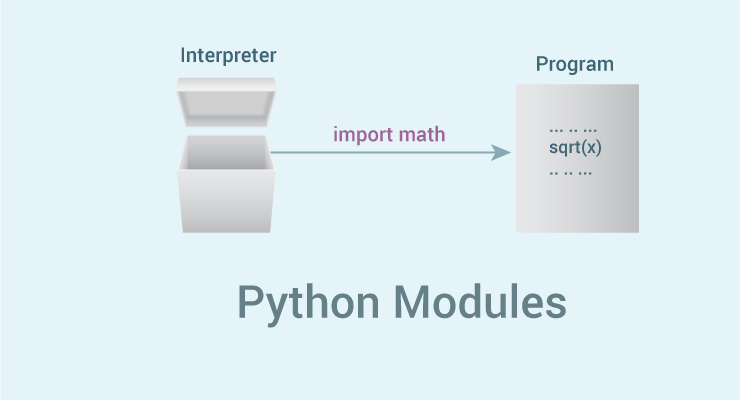
\includegraphics[width=0.50\textwidth]{figures/python_modules}}
	\caption{Python Modules}
	\label{Python Modules}
\end{figure}
\vspace{\baselineskip}

\noindent Modules\par

\vspace{\baselineskip}
\noindent Jika Anda berhenti dari juru bahasa Python dan memasukkannya lagi, definisi yang telah Anda buat (fungsi dan variabel) hilang. Oleh karena itu, jika Anda ingin menulis program yang agak lama, sebaiknya Anda menggunakan editor teks untuk menyiapkan masukan bagi penerjemah dan menjalankannya dengan file itu sebagai masukan. Ini dikenal dengan membuat skrip.\par
\vspace{\baselineskip}
\noindent Seiring program Anda semakin lama, Anda mungkin ingin membaginya menjadi beberapa file untuk memudahkan perawatan. Anda mungkin juga ingin menggunakan fungsi praktis yang telah Anda tulis di beberapa program tanpa menyalin definisinya ke dalam setiap program.\par
\vspace{\baselineskip}
\noindent Untuk mendukung ini, Python memiliki cara untuk menempatkan definisi dalam file dan menggunakannya dalam naskah atau dalam contoh juru bahasa interaktif. File seperti itu disebut modul; definisi dari modul dapat diimpor ke modul lain atau masuk ke modul utama (kumpulan variabel yang Anda akses ke dalam naskah yang dieksekusi di tingkat atas dan dalam mode kalkulator).\par

\vspace{\baselineskip}
\noindent Modul adalah file yang berisi definisi dan pernyataan Python. Nama file adalah nama modul dengan akhiran .py ditambahkan. Dalam sebuah modul, nama modul (sebagai string) tersedia sebagai nilai dari variabel global $ \_ $ $ \_ $ name$ \_ $ $ \_ $ . Misalnya, gunakan editor teks favorit Anda untuk membuat file bernama fibo.py di direktori saat ini dengan konten berikut.\par
\vspace{\baselineskip}
\subsection {More on Modules}

\noindent Modul dapat berisi pernyataan eksekusi serta definisi fungsi.Pernyataan ini dimaksudkan untuk menginisialisasi modul. Mereka dieksekusi hanya untuk pertama kalinya nama modul ditemukan dalam sebuah pernyataan impor. [1] (Mereka juga dijalankan jika file dijalankan sebagai skrip.)\par

\vspace{\baselineskip}
\noindent Setiap modul memiliki tabel simbol pribadinya, yang digunakan sebagai tabel simbol global oleh semua fungsi yang didefinisikan dalam modul.Dengan demikian, penulis modul dapat menggunakan variabel global dalam modul tanpa mengkhawatirkan bentrokan kecelakaan dengan variabel global pengguna.\par

\vspace{\baselineskip}
\noindent Di sisi lain, jika Anda tahu apa yang Anda lakukan, Anda dapat menyentuh variabel global modul dengan notasi yang sama yang digunakan untuk merujuk pada fungsinya, nama modname.itemname.\par

\vspace{\baselineskip}
\noindent Modul bisa mengimpor modul lainnya. Sudah menjadi kebiasaan tapi tidak diharuskan untuk menempatkan semua pernyataan impor di awal modul (atau naskah, dalam hal ini). Nama modul yang diimpor ditempatkan di tabel simbol global modul pengimpor.\par


\vspace{\baselineskip}
\noindent Executing modules as scripts\par
\vspace{\baselineskip}
\noindent Saat Anda menjalankan modul Python dengan\par
\vspace{\baselineskip}
\noindent python fibo.py <arguments>\par

\vspace{\baselineskip}
\noindent Kode dalam modul akan dieksekusi, sama seperti jika Anda mengimpornya, tapi dengan $ \_ $ $ \_ $ name$ \_ $ $ \_ $  set ke "$ \_ $ $ \_ $ main$ \_ $ $ \_ $ ". Itu berarti bahwa dengan menambahkan kode ini di akhir modul Anda:\par

\vspace{\baselineskip}
\noindent if $ \_ $ $ \_ $ name$ \_ $ $ \_ $  == "$ \_ $ $ \_ $ main$ \_ $ $ \_ $ ":\par
\vspace{\baselineskip}
\noindent ~~~ import sys\par
\vspace{\baselineskip}
\noindent ~~~ fib(int(sys.argv[1]))\par

\vspace{\baselineskip}
\noindent Anda dapat membuat file tersebut dapat digunakan sebagai skrip dan juga modul yang dapat diimpor, karena kode yang mem-parsing baris perintah hanya berjalan jika modul dijalankan sebagai file "utama":\par


\vspace{\baselineskip}
\noindent $\$$  python fibo.py 50\par


\noindent 1 1 2 3 5 8 13 21 34\par

\vspace{\baselineskip}
\noindent Jika modul diimpor, kode tidak dijalankan:\par


\noindent >>>\par


\noindent >>> import fibo\par


\noindent >>>\par

\vspace{\baselineskip}
\noindent Hal ini sering digunakan untuk menyediakan antarmuka pengguna yang mudah digunakan ke modul, atau untuk tujuan pengujian (menjalankan modul saat skrip menjalankan test suite).\par


\vspace{\baselineskip}
\begin{itemize}
	\item The Module Search Path
\end{itemize}

\noindent Ketika sebuah modul bernama spam diimpor, penerjemah pertama-tama mencari modul built-in dengan nama itu. Jika tidak ditemukan, maka cari file bernama spam.py dalam daftar direktori yang diberikan oleh variabel sys.path. sys.path diinisialisasi dari lokasi ini:\par

\vspace{\baselineskip}
\noindent $\bullet$  Direktori berisi skrip masukan (atau direktori saat ini bila tidak ada file yang ditentukan).\par
\vspace{\baselineskip}
\noindent $\bullet$  PYTHONPATH (daftar nama direktori, dengan sintaks yang sama dengan variabel shell PATH).\par
\vspace{\baselineskip}
\noindent $\bullet$  Default yang tergantung pada instalasi.\par

\vspace{\baselineskip}
\noindent Setelah inisialisasi, program Python dapat memodifikasi sys.path. Direktori yang berisi skrip yang dijalankan ditempatkan di awal jalur pencarian, di depan jalur perpustakaan standar.\par  
\vspace{\baselineskip}
\noindent Ini berarti skrip di direktori itu akan dimuat alih-alih modul dengan nama yang sama di direktori perpustakaan. Ini adalah kesalahan kecuali penggantinya. Lihat bagian Modul Standar untuk informasi lebih lanjut.\par


\vspace{\baselineskip}
\noindent $``$ Compiled$"$  Python files\par


\noindent Untuk mempercepat pemuatan modul, Python menyimpan versi yang dikompilasi setiap modul di direktori $ \_ $ $ \_ $ pycache$ \_ $ $ \_ $  dengan nama module.version.pyc, di mana versi tersebut mengkodekan format file yang dikompilasi; Umumnya berisi nomor versi Python.\par
\vspace{\baselineskip} 
\noindent Sebagai contoh, dalam rilis CPython 3.3 versi terkompilasi dari spam.py akan di-cache sebagai $ \_ $ $ \_ $ pycache $ \_ $ $ \_ $  / spam.cpython-33.pyc. Konvensi penamaan ini memungkinkan modul yang dikompilasi dari berbagai rilis dan versi Python yang berbeda untuk hidup berdampingan. \par

\vspace{\baselineskip}
\noindent Python memeriksa tanggal modifikasi sumber dari versi yang dikompilasi untuk melihat apakah sudah ketinggalan zaman dan perlu dikompilasi ulang. Ini adalah proses yang benar-benar otomatis.\par  
\vspace{\baselineskip}
\noindent Selain itu, modul yang dikompilasi bersifat platform-independen, sehingga perpustakaan yang sama dapat dibagi antar sistem dengan arsitektur yang berbeda.\par  
\vspace{\baselineskip}
\noindent Python tidak memeriksa cache dalam dua situasi. Pertama, selalu mengkompilasi ulang dan tidak menyimpan hasilnya untuk modul yang dimuat langsung dari baris perintah.\par
\vspace{\baselineskip}  
\noindent Kedua, tidak memeriksa cache jika tidak ada modul sumber. Untuk mendukung distribusi non-source (dikompilasi saja), modul yang dikompilasi harus berada dalam direktori sumber, dan tidak boleh ada modul sumber.\par


\vspace{\baselineskip}
\subsection {Beberapa tip untuk para ahli:}
\vspace{\baselineskip}
\noindent $\bullet$  Anda dapat menggunakan switch -O atau -OO pada perintah Python untuk mengurangi ukuran modul yang dikompilasi. Sakelar -O menghapus pernyataan tegas, tombol -OO menghapus kedua pernyataan tegas dan string $ \_ $ $ \_ $ doc$ \_ $ $ \_ $ .\par
\vspace{\baselineskip} 
\noindent $\bullet$  Karena beberapa program mungkin bergantung pada ketersediaan ini, Anda sebaiknya hanya menggunakan opsi ini jika Anda tahu apa yang Anda lakukan. Modul "Dioptimalkan" memiliki pilihan dan biasanya lebih kecil. Rilis masa depan dapat mengubah efek pengoptimalan.\par

\vspace{\baselineskip}
\noindent $\bullet$  Program tidak berjalan lebih cepat saat dibaca dari file .pyc daripada saat dibaca dari file .py; Satu-satunya yang lebih cepat tentang file .pyc adalah kecepatan pengisiannya.\par

\vspace{\baselineskip}
\noindent $\bullet$  Compileall modul dapat membuat file .pyc untuk semua modul dalam sebuah direktori.\par

\vspace{\baselineskip}
\noindent $\bullet$  Ada lebih banyak rincian mengenai proses ini, termasuk bagan alir keputusan, dalam PEP 3147.\par

